% ============================================================================
% Chi tiết khối _UMobileViTLayer — TikZ diagram
% ============================================================================
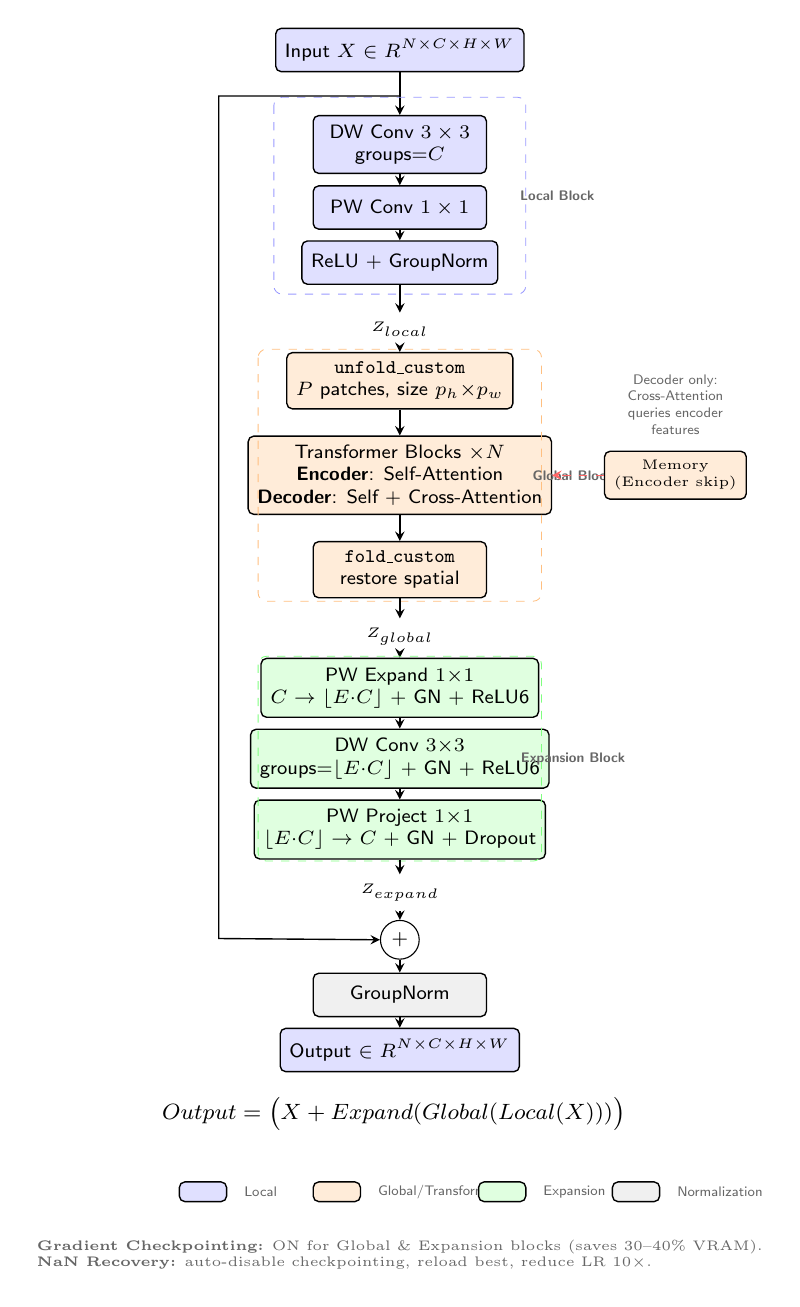
\begin{tikzpicture}[
    block/.style={
        rectangle, draw=black, line width=0.5pt,
        minimum width=2.2cm, minimum height=0.55cm,
        align=center, font=\scriptsize\sffamily,
        rounded corners=2pt,
    },
    local/.style={block, fill=blue!12},
    global/.style={block, fill=orange!15},
    expand/.style={block, fill=green!12},
    norm/.style={block, fill=gray!12},
    arrow/.style={->, >=stealth, line width=0.5pt},
    plus/.style={circle, draw=black, fill=white, inner sep=0pt, minimum size=14pt, font=\scriptsize},
    box/.style={rectangle, draw=black!40, line width=0.3pt, dashed, rounded corners=3pt},
    lbl/.style={font=\tiny\sffamily, text=black!60},
]

% INPUT
\node[local, minimum width=2.8cm] (input) at (0, 0) {Input $X \in \mathbb{R}^{N \times C \times H \times W}$};

% LOCAL BLOCK
\node[local] (dw) at (0, -1.2) {DW Conv $3\times3$\\groups=$C$};
\node[local] (pw1) at (0, -2.0) {PW Conv $1\times1$};
\node[local] (act1) at (0, -2.7) {ReLU + GroupNorm};

\draw[arrow] (input) -- (dw);
\draw[arrow] (dw) -- (pw1);
\draw[arrow] (pw1) -- (act1);

\draw[box, blue!40] (-1.6, -0.6) rectangle (1.6, -3.1);
\node[lbl] at (2.0, -1.85) {\textbf{Local Block}};

\node[font=\tiny\sffamily] (lout) at (0, -3.55) {$Z_{\text{local}}$};
\draw[arrow] (act1) -- (lout);

% GLOBAL BLOCK
\node[global] (unfold) at (0, -4.2) {\texttt{unfold\_custom}\\$P$ patches, size $p_h{\times}p_w$};
\node[global, minimum height=0.8cm] (trans) at (0, -5.4) {Transformer Blocks $\times N$\\\textbf{Encoder}: Self-Attention\\\textbf{Decoder}: Self + Cross-Attention};
\node[global] (fold) at (0, -6.6) {\texttt{fold\_custom}\\restore spatial};

\draw[arrow] (lout) -- (unfold);
\draw[arrow] (unfold) -- (trans);
\draw[arrow] (trans) -- (fold);

\draw[box, orange!50] (-1.8, -3.8) rectangle (1.8, -7.0);
\node[lbl] at (2.2, -5.4) {\textbf{Global Block}};

\node[font=\tiny\sffamily] (gout) at (0, -7.45) {$Z_{\text{global}}$};
\draw[arrow] (fold) -- (gout);

% EXPANSION BLOCK
\node[expand] (exp_pw) at (0, -8.1) {PW Expand $1{\times}1$\\$C \to \lfloor E{\cdot}C\rfloor$ + GN + ReLU6};
\node[expand] (exp_dw) at (0, -9.0) {DW Conv $3{\times}3$\\groups=$\lfloor E{\cdot}C\rfloor$ + GN + ReLU6};
\node[expand] (exp_proj) at (0, -9.9) {PW Project $1{\times}1$\\$\lfloor E{\cdot}C\rfloor \to C$ + GN + Dropout};

\draw[arrow] (gout) -- (exp_pw);
\draw[arrow] (exp_pw) -- (exp_dw);
\draw[arrow] (exp_dw) -- (exp_proj);

\draw[box, green!50] (-1.8, -7.7) rectangle (1.8, -10.3);
\node[lbl] at (2.2, -9.0) {\textbf{Expansion Block}};

\node[font=\tiny\sffamily] (eout) at (0, -10.7) {$Z_{\text{expand}}$};
\draw[arrow] (exp_proj) -- (eout);

% RESIDUAL + OUTPUT
\node[plus] (add) at (0, -11.3) {$+$};
\node[norm] (out_gn) at (0, -12.0) {GroupNorm};
\node[local, minimum width=2.8cm] (output) at (0, -12.7) {Output $\in \mathbb{R}^{N \times C \times H \times W}$};

% Residual connection
\draw[arrow] (input.south) -- ++(0, -0.3) -- ++(-2.3, 0) -- ++(0, -10.7) -- (add.west);

% Main path
\draw[arrow] (eout) -- (add);
\draw[arrow] (add) -- (out_gn);
\draw[arrow] (out_gn) -- (output);

% FORMULA
\node[font=\footnotesize\ttfamily, align=center] at (0, -13.5) {
    $\text{Output} = \GroupNorm\big(X + \text{Expand}(\text{Global}(\text{Local}(X)))\big)$
};

% MEMORY PATH (Decoder only)
\node[global, font=\tiny, minimum width=1.8cm, minimum height=0.4cm] (mem) at (3.5, -5.4) {Memory\\ (Encoder skip)};
\draw[arrow, dashed, red!60] (mem.west) -- (trans.east);
\node[lbl, align=center] at (3.5, -4.5) {Decoder only:\\Cross-Attention\\queries encoder\\features};

% LEGEND
\node[local, minimum width=0.6cm, minimum height=0.25cm, font=\tiny] at (-2.5, -14.5) {};
\node[lbl, anchor=west] at (-2.1, -14.5) {Local};
\node[global, minimum width=0.6cm, minimum height=0.25cm, font=\tiny] at (-0.8, -14.5) {};
\node[lbl, anchor=west] at (-0.4, -14.5) {Global/Transformer};
\node[expand, minimum width=0.6cm, minimum height=0.25cm, font=\tiny] at (1.3, -14.5) {};
\node[lbl, anchor=west] at (1.7, -14.5) {Expansion};
\node[norm, minimum width=0.6cm, minimum height=0.25cm, font=\tiny] at (3.0, -14.5) {};
\node[lbl, anchor=west] at (3.4, -14.5) {Normalization};

\node[lbl, align=left, font=\tiny] at (0, -15.3) {
    \textbf{Gradient Checkpointing:} ON for Global \& Expansion blocks (saves 30--40\% VRAM).\\
    \textbf{NaN Recovery:} auto-disable checkpointing, reload best, reduce LR $10\times$.
};

\end{tikzpicture}
